% ****** Start of file apssamp.tex ******
%
%   This file is part of the APS files in the REVTeX 4.1 distribution.
%   Version 4.1r of REVTeX, August 2010
%
%   Copyright (c) 2009, 2010 The American Physical Society.
%
%   See the REVTeX 4 README file for restrictions and more information.
%
% TeX'ing this file requires that you have AMS-LaTeX 2.0 installed
% as well as the rest of the prerequisites for REVTeX 4.1
%
% See the REVTeX 4 README file
% It also requires running BibTeX. The commands are as follows:
%
%  1)  latex apssamp.tex
%  2)  bibtex apssamp
%  3)  latex apssamp.tex
%  4)  latex apssamp.tex
%
\documentclass[%
 reprint,
%superscriptaddress,
%groupedaddress,
%unsortedaddress,
%runinaddress,
%frontmatterverbose,
%preprint,
%showpacs,preprintnumbers,
%nofootinbib,
%nobibnotes,
%bibnotes,
 amsmath,amssymb,
 aps,
%pra,
%prb,
%rmp,
%prstab,
%prstper,
%floatfix,
]{revtex4-1}

\usepackage{graphicx}% Include figure files
\usepackage{dcolumn}% Align table columns on decimal point
\usepackage{bm}% bold math
%\usepackage{hyperref}% add hypertext capabilities
%\usepackage[mathlines]{lineno}% Enable numbering of text and display math
%\linenumbers\relax % Commence numbering lines

%\usepackage[showframe,%Uncomment any one of the following lines to test
%%scale=0.7, marginratio={1:1, 2:3}, ignoreall,% default settings
%%text={7in,10in},centering,
%%margin=1.5in,
%%total={6.5in,8.75in}, top=1.2in, left=0.9in, includefoot,
%%height=10in,a5paper,hmargin={3cm,0.8in},
%]{geometry}

\begin{document}

%\preprint{APS/123-QED}

\title{Wild Binary Segmentation for multiple change-point detection}% Force line breaks with \\
% \thanks{Working around Binary Segmentation's preference for large signal features}%

\author{Magnus Berg Sletfjerding}
 % \altaffiliation[Also at ]{Physics Department, XYZ University.}%Lines break automatically or can be forced with \\
 % \email{mbs@chem.ku.dk}
% \author{Second Author}%
%  \email{Second.Author@institution.edu}
% \affiliation{%
%  Authors' institution and/or address\\
%  This line break forced with \textbackslash\textbackslash
% }%

% \collaboration{MUSO Collaboration}%\noaffiliation
%
% \author{Charlie Author}
%  \homepage{http://www.Second.institution.edu/~Charlie.Author}
% \affiliation{
%  Second institution and/or address\\
%  This line break forced% with \\
% }%
% \affiliation{
%  Third institution, the second for Charlie Author
% }%
% \author{Delta Author}
% \affiliation{%
%  Authors' institution and/or address\\
%  This line break forced with \textbackslash\textbackslash
% }%

% \collaboration{CLEO Collaboration}%\noaffiliation

\date{\today}% It is always \today, today,
             %  but any date may be explicitly specified
%
% \begin{abstract}
% An article usually includes an abstract, a concise summary of the work
% covered at length in the main body of the article.
%
% \end{abstract}

\maketitle

%\tableofcontents

\section*{Article link}
https://arxiv.org/abs/1411.0858

\section{Introduction}
The accurate treatment and analysis of noisy time series is an ubiquitous challenge across scientific disciplines.
Within the field of single-molecule analysis of biomolecules, low signal-to-noise ratios are a constant problem when fitting models of stochastic change in piecewise-stationary data.

Binary Segmentation is a simple and powerful method for "slicing" data into pieces which come from the same distribution, by finding "change points" in a time series.
While Binary Segmentation is widely utilized in the analysis of time series involving docking and binding on long (s) timescales, it performs significantly less well if the data exhibits multiple change points, especially if they are close to each other.

The article presented proposes an improvement on the classical Binary Segmentation algorithm, in order to analyze data with multiple changepoints accurately.

\section{Binary Segmentation}
The simplest time-series data model can be expressed as

\[X_t = f_t+\varepsilon_t,  t = 1, \textellipsis,T  \]

where \(f_t\) is a one-dimensional signal which has an unknown number of changepoints  \(N\), with unknown locations  \(\eta_1, \textellipsis, \eta_N\), and  \(\varepsilon_t\) is a normal random variable centered at 0.

Classical Binary Segmentation utilizes the CUSUM statistic, which is defined as follows:

\[
\tilde{X}^{b}_{s,e} = \sqrt{\frac{e - b}{n(b-s+1)}} \sum_{t=s}^{b}X_t - \sqrt{\frac{b-s+1}{n(e - b)}} \sum_{t=b+1}^{e}X_t
\]
where \( s \leq b < e \) and \( n = e - s + 1 \).

The Binary Segmentation algorithm finds the first changepoint, \( b_0\) by maximizing \( |\tilde{X}^{b}_{s,e}| \), after which it will look for changepoints in the two new segments of the data.

Finally, the Binary Segmentation stops if the \( |\tilde{X}^{b}_{s,e}| \) for any \( b_0\) is lower than a set threshold.

\subsection{Problems with the Binary Segmentation Algorithm}

\begin{figure}
  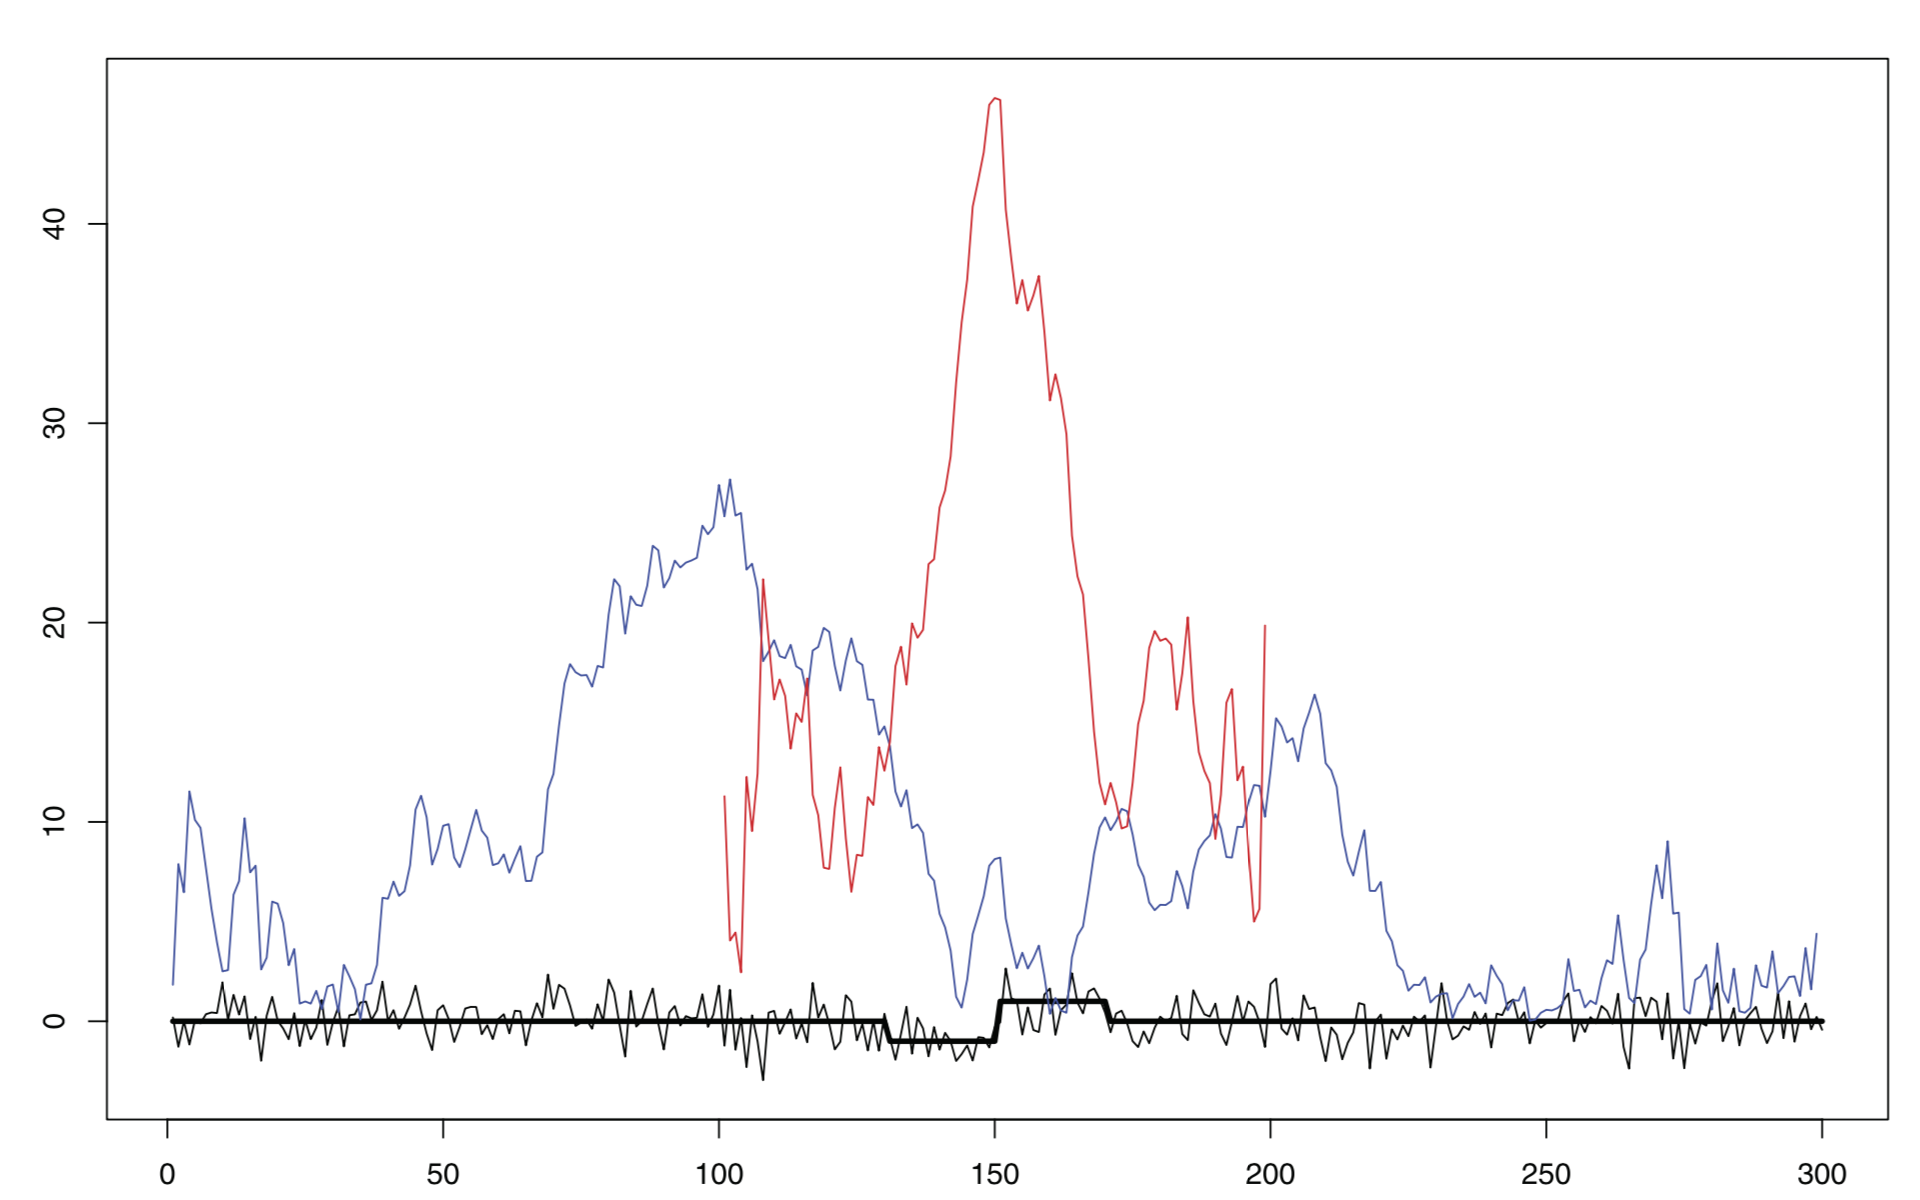
\includegraphics[width=\linewidth]{bsisBS.png}
  \caption{True function in thick black, observed data in thin black, \( |\tilde{X}^{t}_{0,300}| \) plotted in blue and  \( |\tilde{X}^{t}_{101,199}| \) plotted in red.}
  \label{fig_bs}
\end{figure}
\begin{figure}
  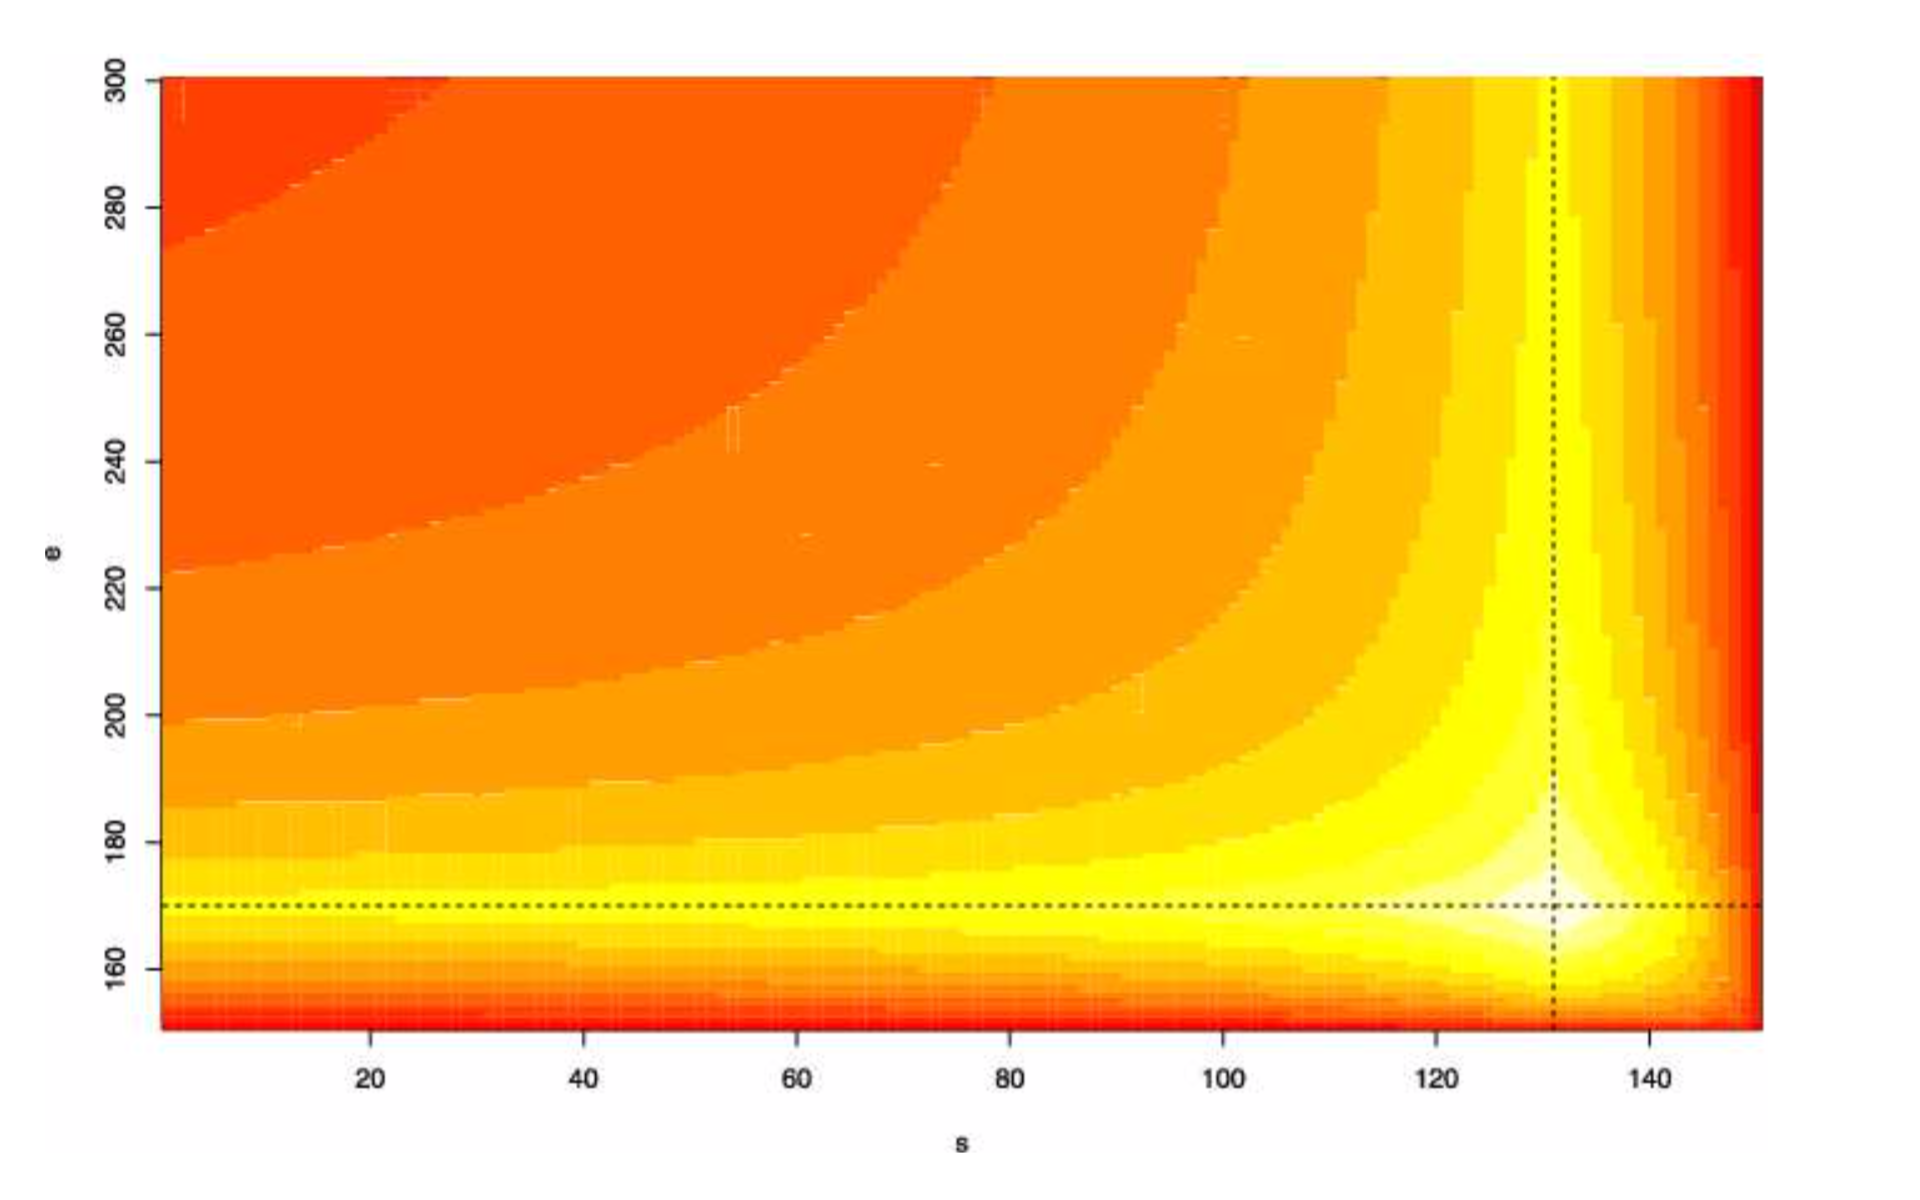
\includegraphics[width=\linewidth]{heatmap.png}
  \caption{Heat map of the values of  \( |\tilde{X}^{t}_{s,e}| \) as a function of s and e.
  Dashed lines indicate the maximum in either dimension, and in this case, the maximum is located at $(s,e)=(131,170)$
  }
  \label{heatmap}
\end{figure}

As seen in Figure \ref{fig_bs}, a large window ( e.g. calculating \( |\tilde{X}^{t}_{0,300}| \) ) will cause a misrepresentation of the data, and $b_0$ is estimated to be at $t=100$.
However, with a smaller window, the maximizer accurately finds the change point at $t=150$.
This point is further illustrated by Figure \ref{heatmap}, where the values clearly show that the window size to find this particular change point is much smaller than 300 frames.
The need for a more robust method for estimating the peaks is therefore obvious.


\section{Wild Binary Segmentation}
Wild Binary Segmentation works in a similar manner as Binary Segmentation, but differs in the way it finds \(b_0\).

For Wild Binary Segmentation, \(F_T^M\) is a set of $M$ randomly sampled intervals $[s_m,e_m], m=1,\textellipsis,M$ where $[s_m,e_m]$ have been drawn from ${1,\textellipsis, M}$.

While Binary Segmentation uses a simple maximization of \( |\tilde{X}^{b}_{s,e}| \) over the entire data, Wild Binary Segmentation instead maximizes
\( |\tilde{X}^{b}_{s_m,e_m}| \), hence forming a 2-dimensional space to maximize, with m on one axis, and b on the other.

Like the Binary Segmentation algorithm, the Wild Binary Segmentation also stops if \( |\tilde{X}^{b}_{s,e}| \) is lower than a set threshold.



\section{Performance}

\begin{figure}[t!]
  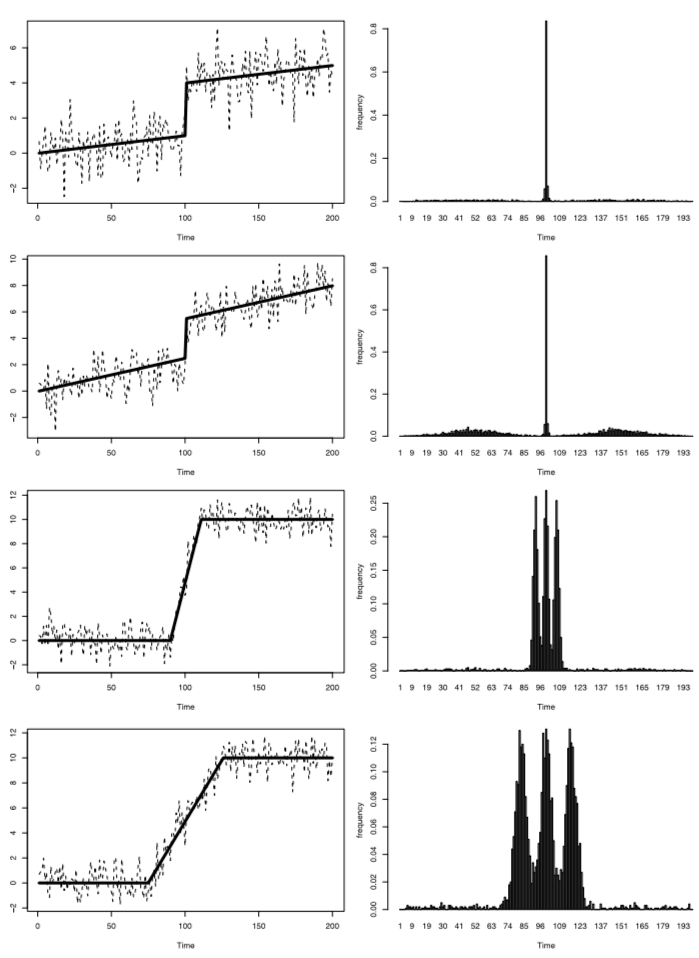
\includegraphics[width=\linewidth]{traces.png}
  \caption{
  Left: linear trend data (spots) and true functions (black lines).
  Right: frequency histograms of the found change points.
  }
  \label{traces}
\end{figure}


The Wild Binary Segmentation was compared to a series of publicly available datasets, and was shown to outperform classical Binary Segmentation in all cases.
As seen in figure \ref{traces}, Wild Binary Segmentation still misclassifies the middle of a linear (i.e. not instant) transition.
Even so, the algorithm still manages to find the "true" change points, asserting its advantage over typical Binary Segmentation.


\section{Conclusion}
The Wild Binary Segmentation algorithm is a significant improvement upon the classical Binary Segmentation algorithm.
While it does not perfectly find all change points, and misclassifies some points, it still does not mask points in the same way as the Binary Segmentation algorithm does, as its implementation ensures stochastic selection of segments.
This prevents agains successive errors being repeated, as the repetition of random draws allows the user to withdraw a distribution of results, if they remember to rerun the experiments a series of times.



\end{document}
%
% ****** End of file apssamp.tex ******
